\documentclass[format=siggraph, review=true]{acmart}
\usepackage{graphicx}
\acmConference{Computation + Journalism Symposium}{October 2017}{Chicago, IL}
\title{Machine Assisted Dossiers}
\author{Forest Gregg}
\affiliation{DataMade}
\email{fgregg@datamade.us}
\author{Jean Cochrane}
\affiliation{DataMade}
\email{jean.cochrane@datamade.us}
\author{Timothy McGovern}
\affiliation{O'Reilly Media}
\email{timmymcg@gmail.com}
\begin{document}


\begin{abstract}One of the great disappointments of big data is that so much
  of it is bad data. It is unreliable, ambiguous, and
  contradictory. Developing an accurate image of the world still
  requires discernment, sorting, and judgment.

  We are still are only beginning to building technologies that are
  complementary to these human capacities--allowing for
  scale.  In this paper, we present the capabilities we believe an
  adequate knowledge system must have, drawing heavily from the field
  of genealogy and our own work modeling international security forces
  and campaign finance.

  We'll discuss the overall requirements for such a system and try to envision its user experience and its data architecture; we'll also survey where currently available technologies can fill in the gaps between the two. 
\end{abstract}

\maketitle

Most of the time, investigative journalists use data and documents
that were not made for them. The material that they FOIA, scrape, get
leaked, download from data portals, or dig up from the archives
were not made for journalists or intended to help answer the
questions she is reporting.

In order to do their work, journalists have to struggle to get access
to documents or administrative data; manage large collections of
source files; extract the relevant information; identify ambiguous
references; and reconcile conflicting claims.

That journalists accomplish these tasks and relatively quickly is a
testament to their skills as researchers. These skills though are
private and focused on the investigations at hand. The work does not
accumulate a store of knowledge that can be reused by future
journalists for new investigations.

The promise of computers, meantime, is to offer speed (enabling the
analysis of larger corpora of source material), scale (enabling the
analysis of larger webs of interrelated facts), and memory (enabling
knowledge to be stored and shared, whether for reproducing an analysis
or for bringing the knowledge to bear on a new problem).

Though journalists and newsrooms would benefit from building shared
dossiers of the key people and organizations in a beat, this is not a
common practice. The reasons for this are various, but we believe a
substantial barrier is that existing tools do not provide immediate
benefits to a journalist in the middle of an investigation. It may be
very helpful for a journalist to look up what the news room already
knows about a city councilor in an internal wiki, but adding new
content to the wiki is just an additional chore. 

At DataMade, we have been building and researching knowledge
management systems that can help the investigators in the many stages
of research and which, almost as a byproduct, produce shared dossiers
of people and organizations. In this paper, we discuss the
capabilities that a well designed system should possess, from the
perspective of information architecture and end-user experience.

\section{Existing Tools}
Existing knowledge management systems prioritize flexibility for the
individual researcher over general utility for a team, or for a wider
audience. 

When individual researchers are afforded flexibility to organize
information as they please, the information is almost always put into
a form that suits the researcher's personal preferences and their
current research topic. Considerable work is required to
recontextualize the information into a form that is convenient for
other uses. Conversely, when data must be organized to support the
general uses and users, researchers usually lose capacity for
tolerating ambiguity, and the tools is not perfectly adapted to the
current project.

Here, we consider the affordances and limitations of a few of the most
popular tools for knowledge management in research contexts.

\begin{description}
  \item [Notecards] Collecting and organizing analog files remains
    a popular research method, for good reason. Using notecards, an
    individual researcher is free to organize and reorganize a
    knowledge system however she pleases. Notecards neatly illustrate
    the tradeoff between flexibility and utility involved in designing
    a knowledge system: they offer total control to the individual
    researcher at great cost to the general public, for whom the system
    must be painstakingly translated to be of any use at all.

  \item [Scrivener] Composition tools like Scrivener port the visual
    and mechanical metaphors of analog research methods to digital
    contexts. With these tools, information can be recorded in digitized
    form, but it is still completely unstructured. The individual
    researcher is able to keep track of more and more different kinds
    of information, but translation is still required in order for others
    to make sense of it.

  \item [Wikis] In contrast to notecards and digital composition tools,
    wikis prioritize the needs of a collective of stakeholders over the
    individual researcher. Information is sometimes structured and
    attached to specific sources, and the process that produced the
    knowledge can be preserved in discussion forums. In a wiki, however,
    individual researchers lose a great deal of power in order to create
    value for the collective: knowledge is subject to collective approval,
    and conflicting truth claims must be reconciled fully and immediately.
\end{description}

\section{Scope Conditions}
In order to provide more support for journalists and other
researchers, a system must be designed for a defined universe of
knowledge to manage -- the types of organizations, persons, and
events; the attributes of those entities; and the relations amongst
them.

With these set, the designer of the system can identify source
material with potential relevance, what pieces of information that
will be important in the source material, what facets of the
information will be useful to index, and what types of claims are
congruent or incompatible.

The more defined the field of knowledge, the more that information
technology can aid the production of that knowledge. However, given
the current costs of building, a limited field of knowledge is not
sufficient. These types of systems should only be built where three
conditions are met. First, there is fairly narrow knowledge area that
has wide and durable interest. Second, the number concrete instances
of knowledge is much larger than one person can manage using private
skills. Three, there is a large corpus of primary source material that
can be used to develop concrete knowledge in a repeatable and
separable manner.

Some examples include:

\begin{description}
  \item [Geneology] Who were the parents of whom. When and where was a person
    born and when and where did they die.
  \item [Corporate Beneficiaries] Who ultimately owns or controls an
    organization, which may be owned by a chain of shell organizations
  \item [Security Forces] What is the organizational structure of
    security forces. Who are the commanding officers of units and
    what has been their careers.
  \item [Campaign Finance] Who, ultimately, gave money to which
    political campaigns, even through intermediaries.
  \item [Human Rights Violations] Who and how many people have been
    killed in an armed conflict
  \item [Customer Resource Management] The nature and relationships of individuals and organizations; the history of contacts between them. 
\end{description}

Consider three different organizations, each working in one of these problem
domains, each with separate missions but similar sets of problems:

Security Force Monitor is a nonprofit based out of Columbia University
with the mission of tracking of security force activity in conflict areas
around the world. Maintaining a robust knowledge system is a key part of
their mission, but it is a difficult task: keeping track of security forces
requires keeping track of large quantities of ambiguous
information—information that has been retrieved from unreliable sources,
primarily secondary news reports, and that is then adjudicated by staff
members who lack authoritative context. For any given assertion about a
human rights violation to be credible, the knowledge system must know
where each piece of information came from, which researcher catalogued it,
and the degree of confidence the researcher had in the assertion. Yet for
the system to be useful to an audience outside of the internal research
team, it must also be capable of adjudicating conflicting claims and
presenting a structured view of the security forces and the incidents
they have been involved in.

Invisible Institute is a nonprofit media organization in Chicago that
reports on misconduct in the Chicago Police Department (CPD). Following
their legal victory in Kalven v. City of Chicago in 2014, which opened
up over 56,000 complaints against CPD officers to the public, they have
released a database of complaint records to the public with detailed
demographic information about complainants and officers involved in
alleged misconduct. The organization would like to be able to produce
a dossier of CPD officers in order to to link these complaints to other
kinds of misconduct records, but the source records that they FOIA from
the CPD and the City of Chicago are typically difficult to parse, and
lack the unique identifiers that would allow them to unambiguously
assign responsibility for incidents.

FamilySearch is a service provided by the Church of Latter-Day Saints
that seeks to build detailed genealogies using demographic records.
The service sources much of its information from old census records,
which are OCRed and then interpreted by staff members, but it also allows
users to upload their own records and contest genealogies recorded by the
system. Every claim must be tied to a specific record, and contested
assertions are eventually adjudicated.

As we describe the necessary features of machine-assisted dossiers, we will
refer back to the problems and solutions that these three organizations
engage with in their attempts to build comprehensive knowledge systems.

\section{Document Management}
The system must have the capability to collect the source material
which will be the evidence to support the development of
knowledge and make those materials convenient for the purposes of
research. The set of problems here are largely covered under the field
of document management and there already exists many excellent tools
for this portion of the task. Within journalism, the prominent
examples include DocumentCloud, aleph, and the PANDA project.

For our purposes, we are using ``document'' to mean any type of source
material. They are most often different types of files: word
processing documents, PDFs, markup, spreadsheets, etc. They could
include audio testimony, news articles, or FOIAed documents.

Beyond storage, the three key capabilities for document management
portion of the system is to capture the provenance of source material;
converting the source material into convenient formats; and indexing
the documents in support of research.

\subsection{Provenance}
As the knowledge developed within the system ultimately depends upon
source documents, the provenance of those documents must be
recorded. Who or what (if it was an automated scraper) collected the
material, when, from what original location. The original forms of the
documents must be preserved.

\subsection{Formatting}
Often, source material is not in a convenient format for computer
processing. A file may be in an awkward or proprietary format, or a
document may only be collected as scanned image. As part of the
research process, the material may be converted to a form that allows
for easier processing. Sometimes this conversion is unproblematic,
like for many file format conversions. Sometimes, the conversion is
very error prone such as OCRing a scanned document or human
transcription of audio recordings.

Regardless, the details about the conversion need to be recorded ---
who or what did the conversion and when. If the process was done by
computer, steps must be taken to ensure that the conversion is
completely reproducible. As technologies or other capabilities
improve, the journalist or researcher may want to reconvert existing
documents and conversion metadata supports this.

\subsection{Indexing}
Finally, appropriately formatted documents should be indexed for the
next stage of research. While the systems should to full-text indexing
to allow for flexible searches, the system should also attempt to
index the documents on facets relevant to the target knowledge
area. This means that the system should attempt to identify references
within a document to the types of person, organizations, places, and
events that the overall system is concerned with.

If the source material is already highly structured, this can be
simple. However, if the material is free text, then the system should
be attempt to identify references using Named Entity Recognition
techniques. 

Indexing is the most basic form of computer analysis of documents. It
enables non-trivial analysis of topics and relevant entities through
simple counting and co-location analysis, and when combined with
minimal provenance data (chronology), can provide evidence of change
over time. Indexing also provides the basis for building a databases
of named entities.

\section{Entity Management}

Once we have secured our documents, regularized them, and indexed
them, producing a searchable list of entities is rewarding both
immediately and in the long term. ``What do we know about Jane Tye?''
is a question that can be usefully answered with a keyword-in-context
(KWIC) search, even when the search produces hundreds of hits. Entity
management also can entail using machine learning techniques to
preliminarily classify entities. This may entail sifting out
individuals from organizations, or well-connected individuals from
peripheral ones, but we can start to see the basis for
machine-assisted analysis of large data sets.

\section{Claim Management}
Once the documentary base is prepared, the work of extracting claims
about the world from those documents, resolving those claims to
reference particular entities, and reconciling conflicting claims can
begin. Unlike document management, the practices for what we call
``claim management'' are still developing.

\subsection{Extracting Claims}
Given a source document, a journalist will extract claims relevant to
the entity of interest. If they are researching campaign finance, they
might be interested in the extracting the claim that ``John Smith''
gave \$500 to ``Citizens for Better Citizens'' on December 11, 2017
from a financial disclosure form of the ``Citizens for Better
Citizens'' political action committee.

While system should allow the journalist to extract the claims in the
most natural, practicable manner, the system should decompose compound
claims into simpler claims. For example, the above
claim could be broken down as follows:

\begin{itemize}
\item ``John Smith'' made a contribution to this committee
\item ``John Smith'' made a contribution during the reporting period of this disclosure
\item ``John Smith'' made a contribution to this committee on December 11, 2017
\item ``John Smith'' gave this committee \$500
\item somebody gave this committee \$500 during this reporting period
\item somebody gave this committee \$500 on December 11, 2017
\end{itemize}

Extracting claims is effortful. While full compound claims are often
incorrect in some particular, elements of the claim can often be
maintained and this decomposition preserves some of the initial work.

The types of claims that can be recorded are those that the system has
been designed to handle. The system must capture and preserve data on
who or what extracted the claim and when this extraction occurred.

\subsection{Resolving Claims}
In the cases we deal with, there is almost always ambiguity about
which particular entity a claim in a document is about. While a
journalist will believe they are extracting a claim about a particular
person or organization, they can find that they have been
mistaken. Using the above example, a journalist can mistakenly
attribute a campaign contribution to the wrong ``John Smith.''

The knowledge system must allow for this type of ambiguity by avoiding
modeling extracted claims as claims about particular
instances. Internally, an extracted claim attached to a particular
dossier would be modeled as two related claims. The first is the one
extracted from the document: `A person with the name ``John Smith''
gave \$500 to this committee.' The second claim is `The person who is
referenced in the extracted claim is the person who this system
uniquely indexes with the unique identifier ``1313515'''

If claims about particularly people are split in this way, then
extracted claims can be re-assigned to the correct entities as the
journalist develops a more accurate picture.


\subsection{Reconciling Claims}
Since the knowledge systems work within limited fields of knowledge,
the system designers can elaborate a model of how the this portion of
the world should operate. This can allow for the flagging of claims
that are logically incompatible. For example, campaign committees have
founding dates, so there should be no contributions from a campaign
committee before it was founded. 

With or without the help of system, the journalist must decide which
claims are compatible and decide which, if any, they want to
accept. The system must be able to record the journalist's belief about
the validity of a claim about a particular person or
organization. These decisions should be reversible.

\section{Example Designs}
Researcher use of the system will be organized around number of tasks:

\begin{description}
\item[Creating an Entity] The user must be able to create new profile
  page for an entity, either from scratch or through accepting a
  system proposed entity
\item[Viewing information on an Entity]
\item[Adding and editing information about an entity] The system must
  record all changes made the an entities attribute and maintain a
  complete audit log. All modifications to an entity should be tied to
  a document. This includes claims that 
\item[Search entities] The user must be able to search for profiles of
  existing entities using full text search or faceted search
\item[Search documents] The user must be able search source documents
  using full text and faceted search
\item[View details about Document] The user must be able to view any
  metadata about any individual document. The raw source material
  itself, i.e. scanned image. If the system has attempted
  to extract data from the document, this should be visible next to
  the source document.
\item[Correct extracted document information] If the system attempts
  to extract data from documents, the system should allow users to
  correct incorrect extractions. This should be fully auditable.
\item[View high order structure]
\item[Merge entities]
\end{description}

In order to assist the user, the system must be responsible for the
following tasks:

\begin{description}
\item[Propose potentially relevant documents] When relevant to the
  user's tasks the system should propose documents that might
  contain relevant information about an entity
\item[Propose possible entities] When relevant to the user's task, the
  system should propose that the existence of an entity that seems to
  referred to in one or more source systems
\item[Warn of logically conflicting information] When users enter in
  information about an entity that is logically impossible, the system
  should warn the user.
\end{description}

We now provide example interfaces for how these tasks can be
accomplished.

\section*{Family Search Implementation}
This tasks are best elaborated in a discussion of concrete
implementation. The most sophisticated implementation we have seen in
the FamilySearch.com, a geneology site operated by the Church of
Latter Day Saints. 

\subsection*{Person Profile Page}
FamilySearch has a profile page for current person in their
system. The page contains an impressive amount of information and
functions without overwhelming the user.

\begin{figure}[h]

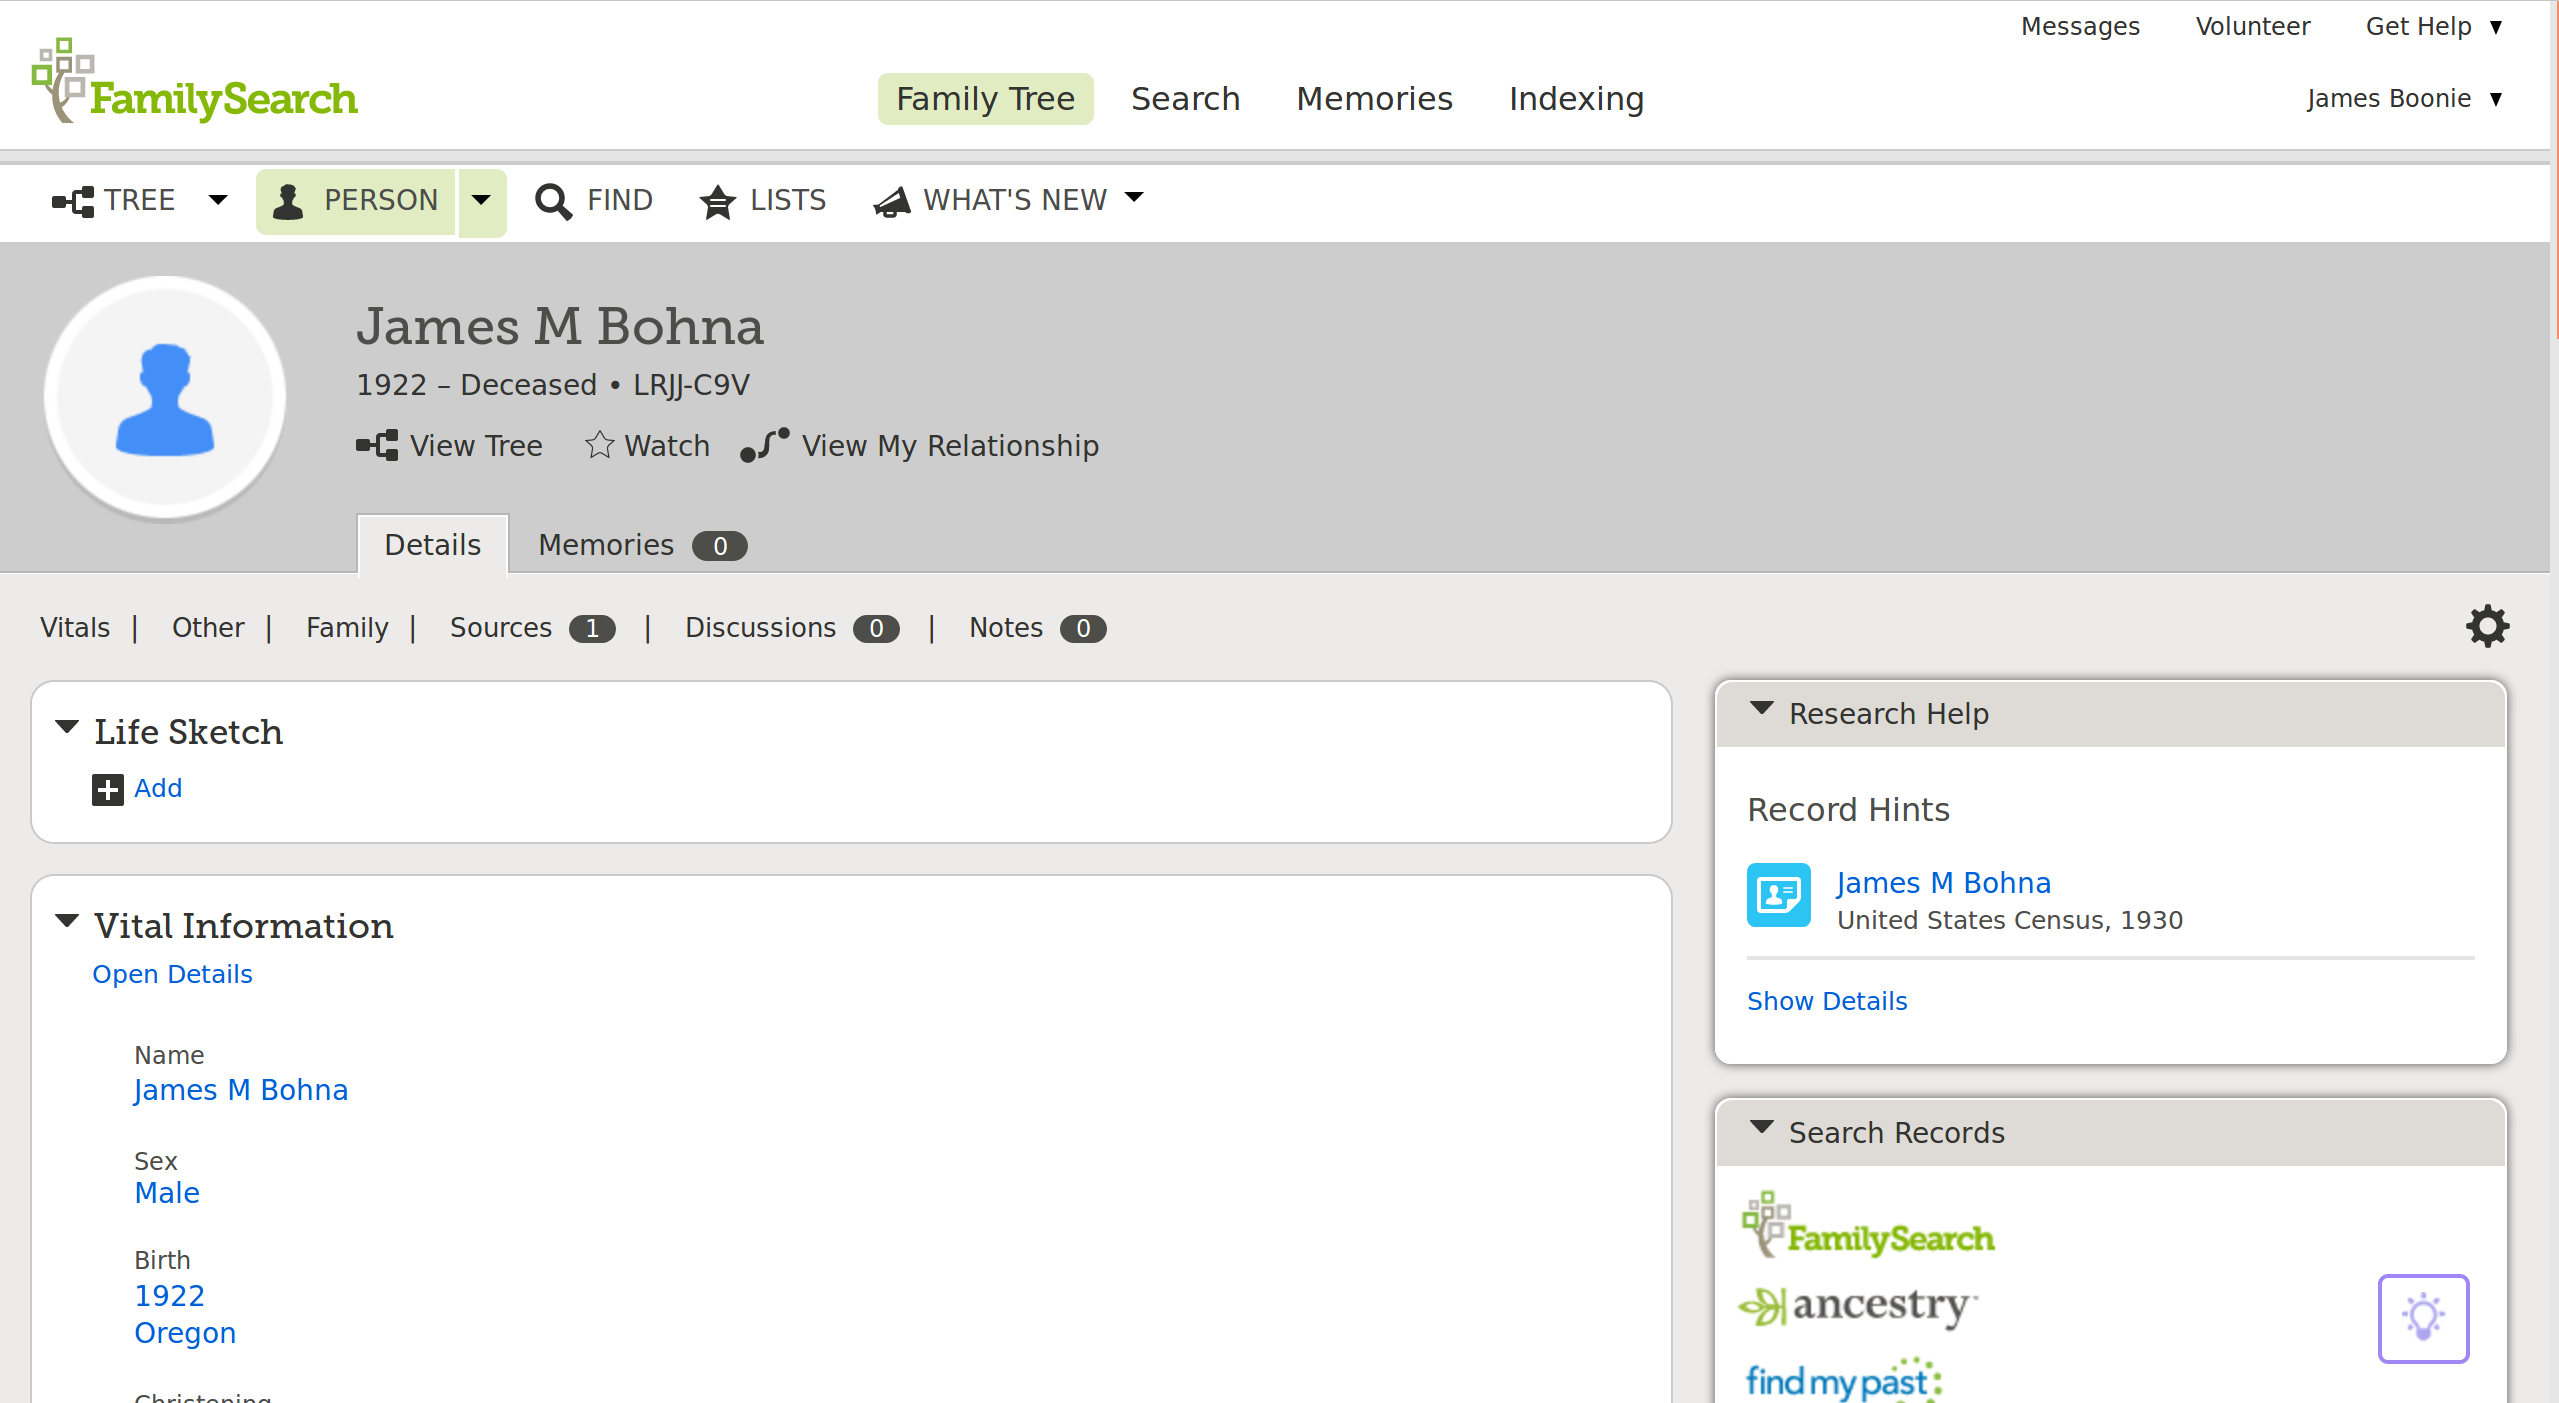
\includegraphics[width=\columnwidth]{images/familysearch/person-detail-1.png}

\caption{FamilySearch Person Profile Page}
\end{figure}

The site includes all the information that users have claimed as true
about this person. Clicking on piece of information shows the he
details about the claim for inspection --the user that made the
claim, when the claim was made, and the source record that supports
the claim (Figure~\ref{fig:name-detail}).

\begin{figure}[h]
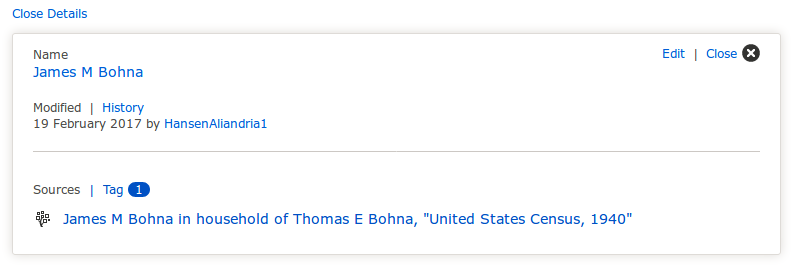
\includegraphics[width=\columnwidth]{images/familysearch/name-detail.png}
\caption{Claim Details}
\label{fig:name-detail}
\end{figure}

New claims can be made in this detail view. The system will recorded
the user that made the claim, when it was made, and the justification
for the claim (Figure~\ref{name-edit}).

\begin{figure}[h]
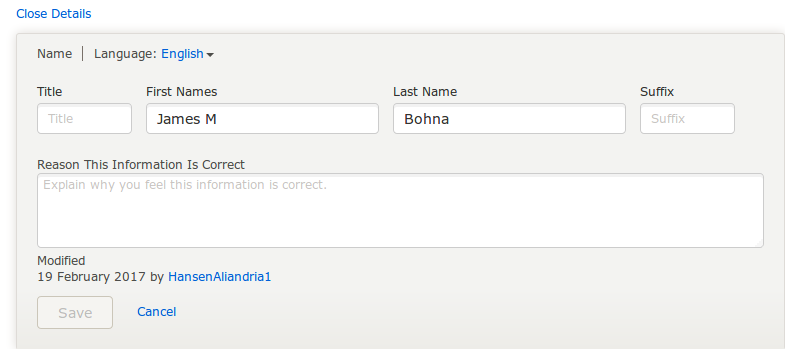
\includegraphics[width=\columnwidth]{images/familysearch/name-edit.png}
\caption{Adding Claims}
\label{fig:name-edit}
\end{figure}

The profile page also can suggest source records that might be
relevant to this person (Figure~\ref{fig:record-hint}).

\begin{figure}[h]

\includegraphics[width=\columnwidth]{images/familysearch/record-hint.png}
\caption{Source Record Suggestions}
\label{fig:record-hint}
\end{figure}

If the claims made about a person are logically impossible or just
very unlikely, the profile page shows these concerns
(Figure~\ref{fig:data-problems}). FamilySearch allows users to
enter logically impossible claims, but warns viewers of the
page. Another system could decide to not allow users to enter
logically impossible claims.

\begin{figure}[h]
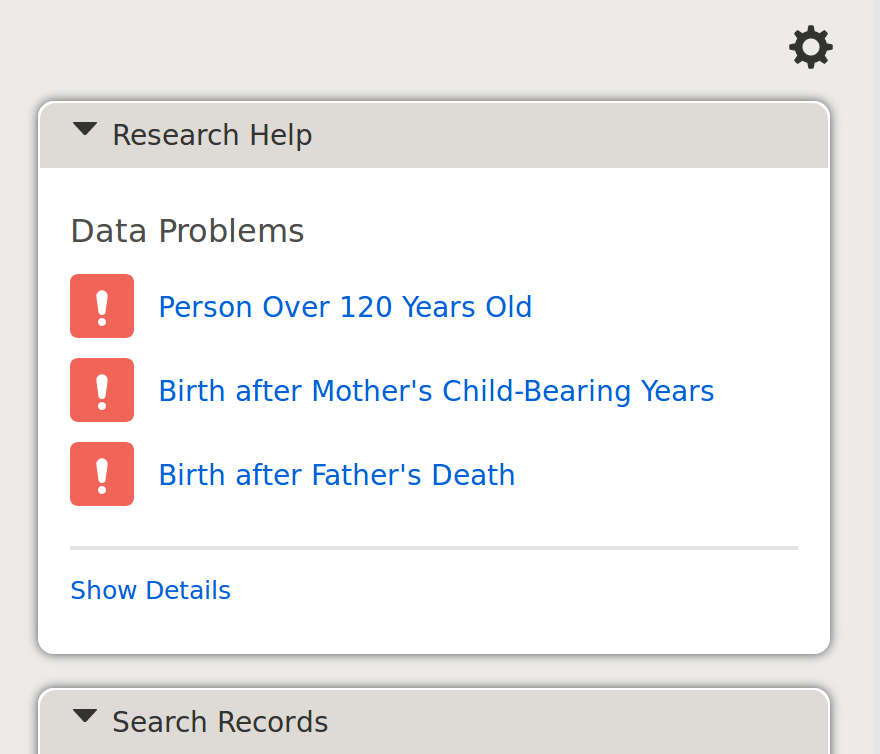
\includegraphics[width=\columnwidth]{images/familysearch/data_problems_detail.png}
\caption{Unlikely or Impossible Claims}
\label{fig:data-problems}
\end{figure}

\subsection*{Record Search and Interface}
While users can directly make claims about persons on profile pages,
the system strongly encourages people to make claims about people
through the source record detail interfaces.

Working with source records starts with the search page. The users can
search by name, location of important life events, or the names of
important relations to the focal person
(Figure~\ref{fig:search-record}).

\begin{figure}[h]
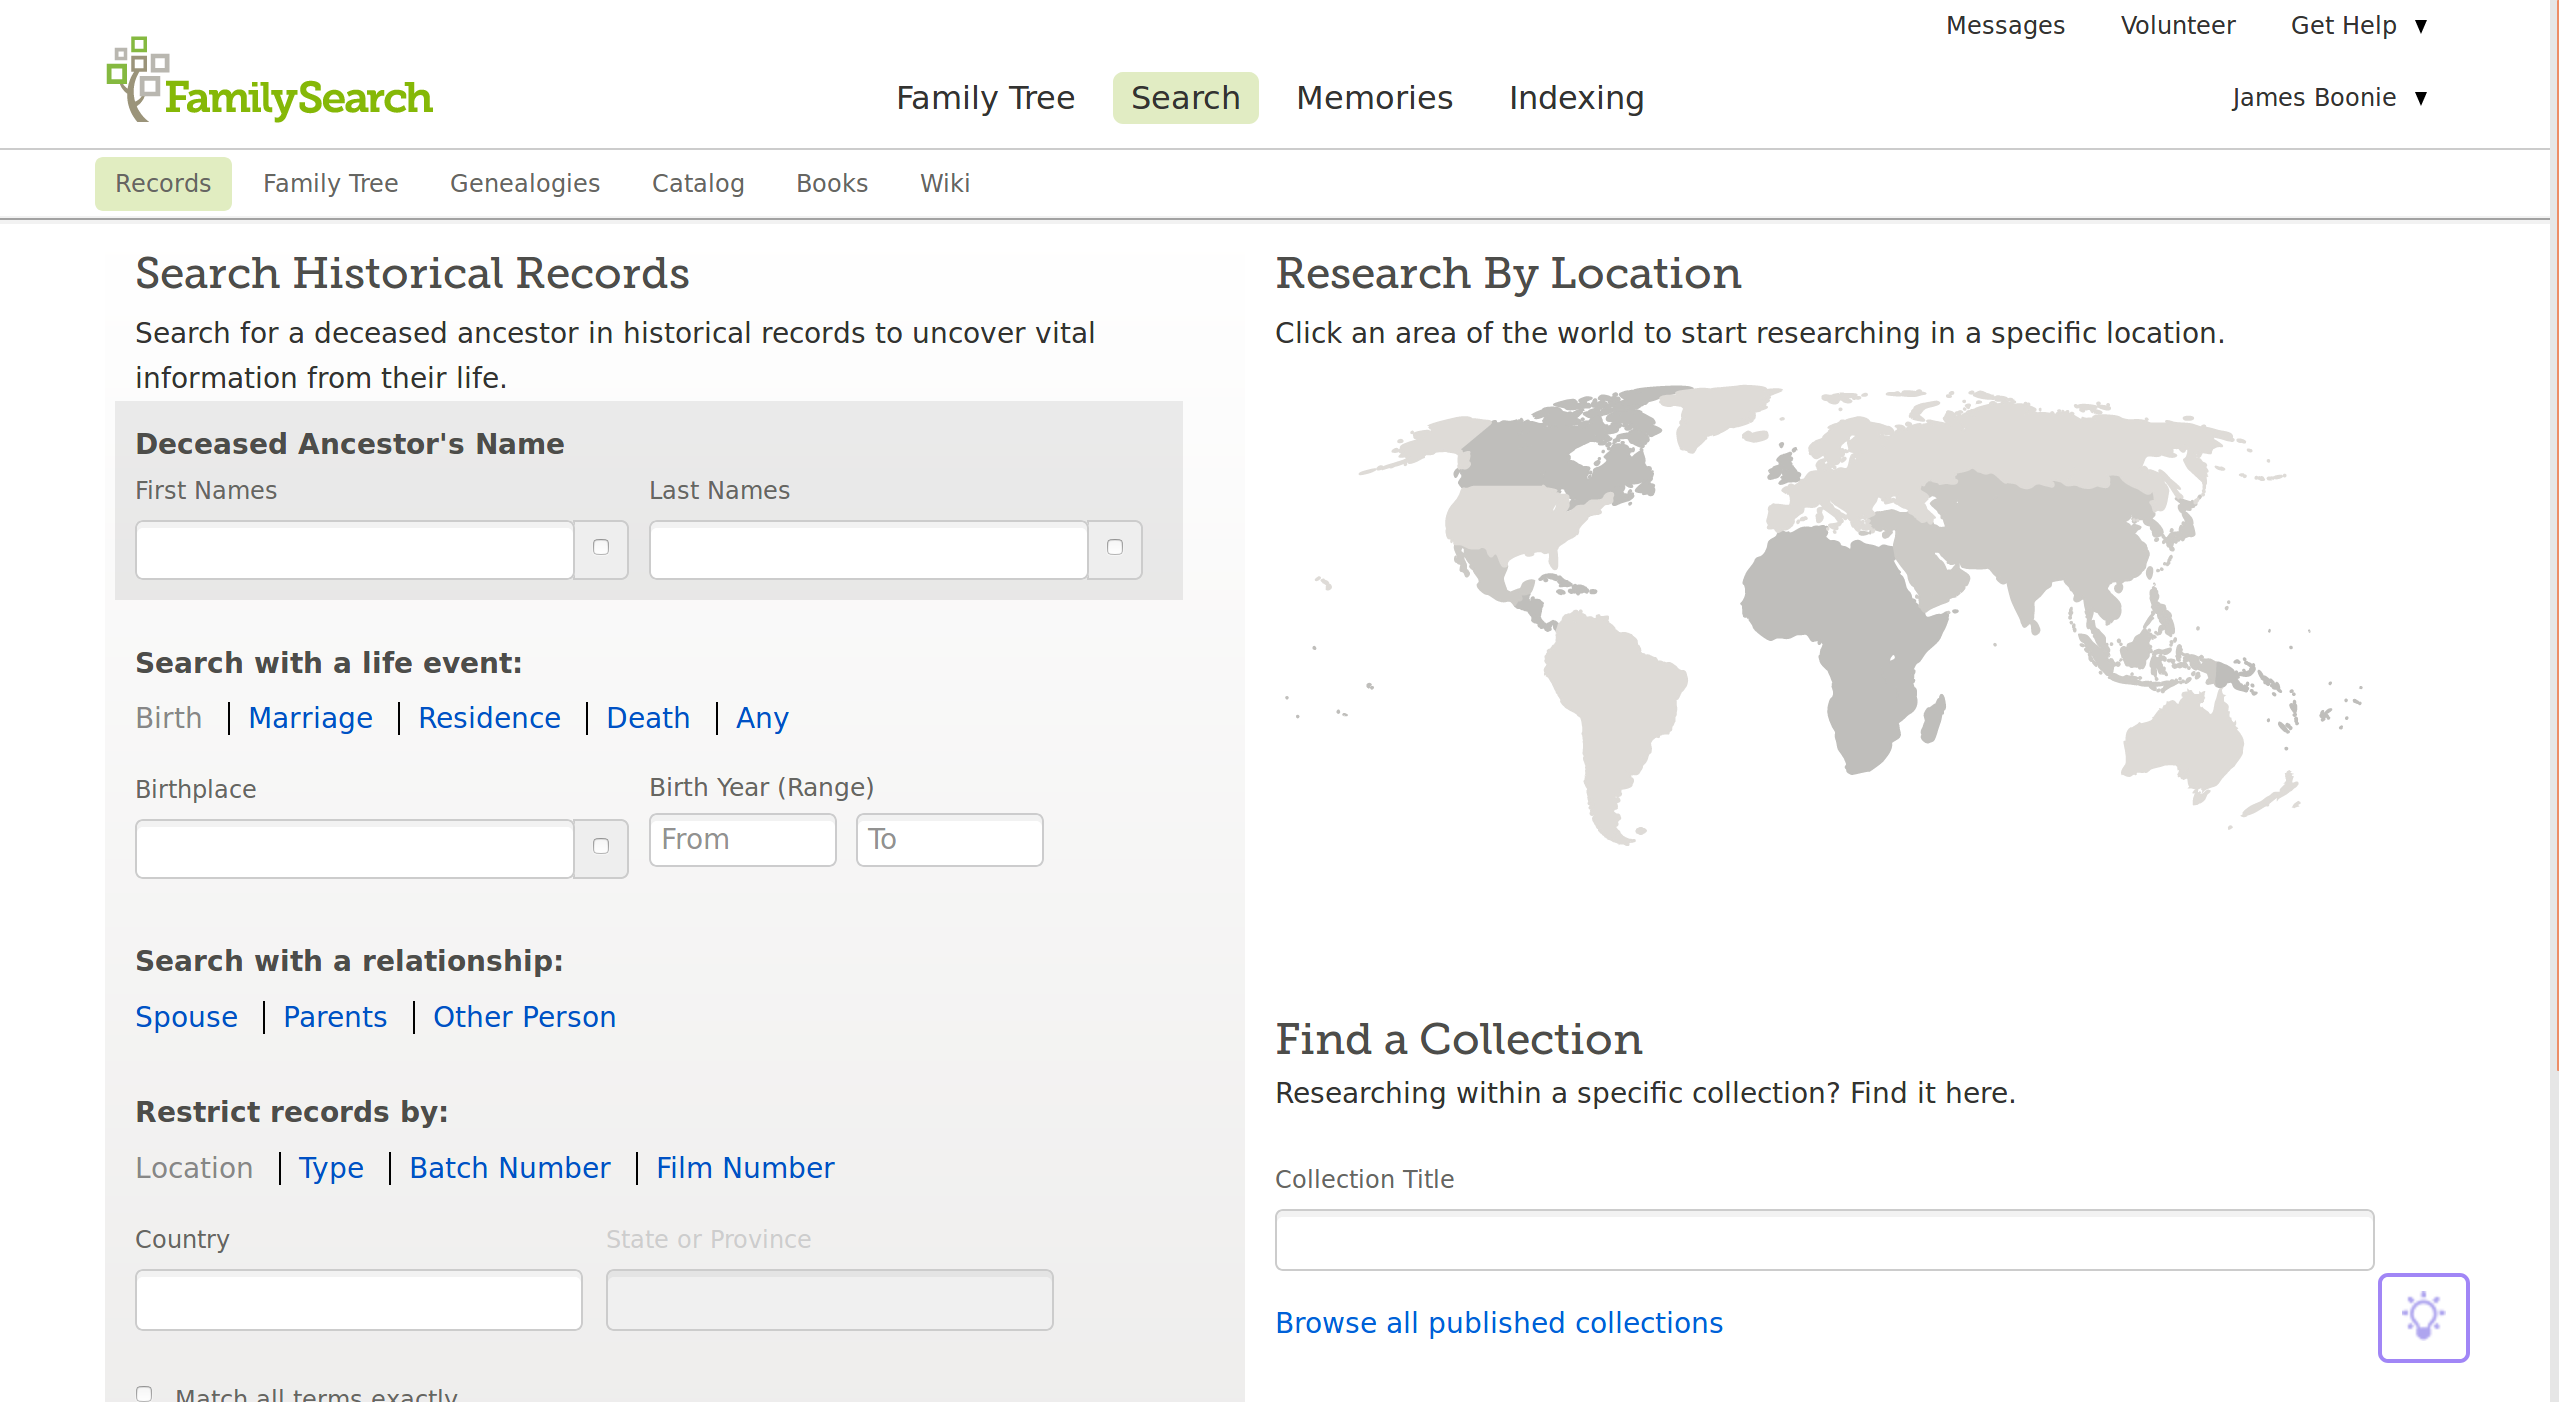
\includegraphics[width=\columnwidth]{images/familysearch/search-records.png}
\caption{Search}
\label{fig:search-record}
\end{figure}

The search results show the name and other information that have been
extracted from the source record. Clicking on a result shows details
about the source document, all information extracted from the source
document related to the focal person, and a link an image of the
source document.

\begin{figure}[h]
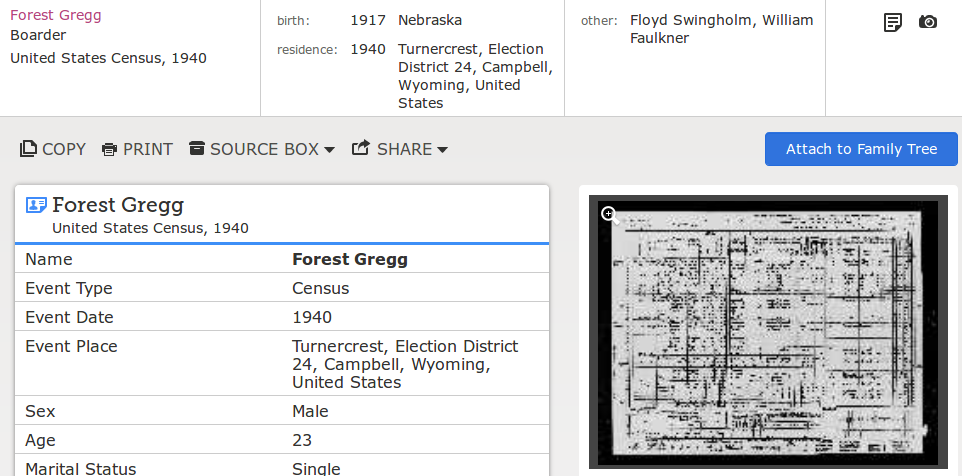
\includegraphics[width=\columnwidth]{images/familysearch/search_result_detail.png}
\caption{Search Detail}
\label{fig:search-details}
\end{figure}

If the user decides that a record is relevant to her person of
interest, she will click the ``Attach to Family Tree'' button, which
takes the user to a ``source linker'' page. Here, she sees a two
column view where she can align references that appear in a record to
persons with existing profile pages.

\begin{figure}[h]
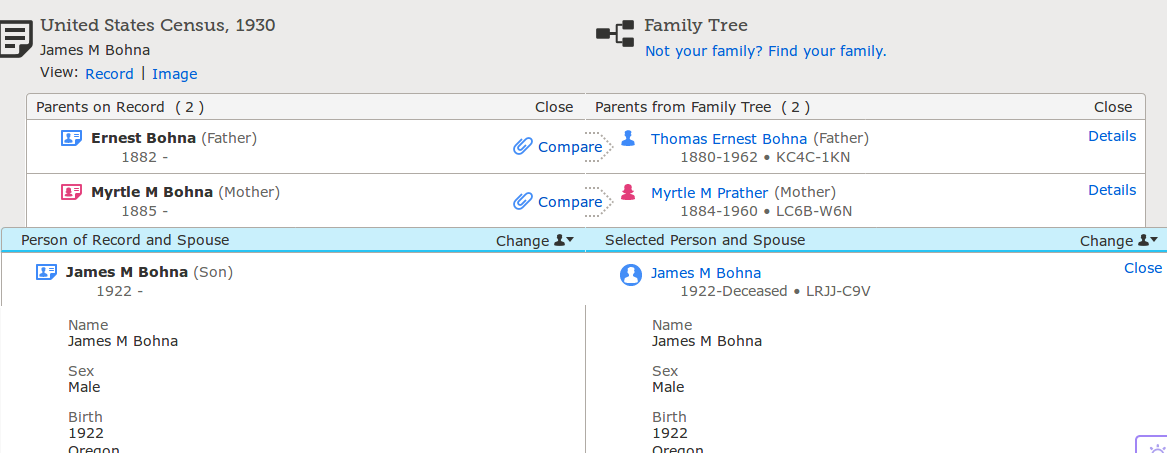
\includegraphics[width=\columnwidth]{images/familysearch/source_linker.png}
\caption{Source Linker}
\label{fig:source-linker}
\end{figure}

For each reference, she can decide to link it to a person or not. If a
piece of information is in the record but not in the profile, it can
be added. Information added here will show up on the profile page, and
be linked back to the source record.

\begin{figure}[h]
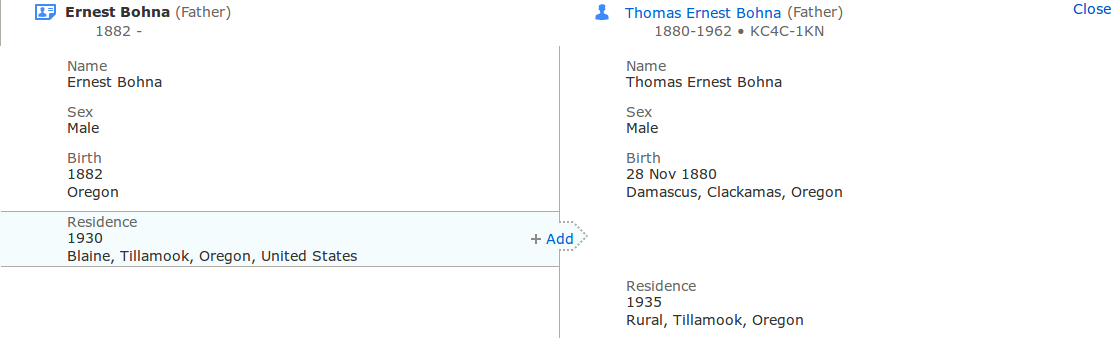
\includegraphics[width=\columnwidth]{images/familysearch/add_info.png}
\caption{Add Information from Source Record}
\label{fig:source-linker}
\end{figure}

While FamilySearch.org has many other sophisticated features, the last
we'll touch on is the view they make available for the connections
between persons. In addition the person focused information available
on a profile page--parents, siblings, children, and
spouse--the site also provides a network view of these relations as
family tree.

\begin{figure}[h]
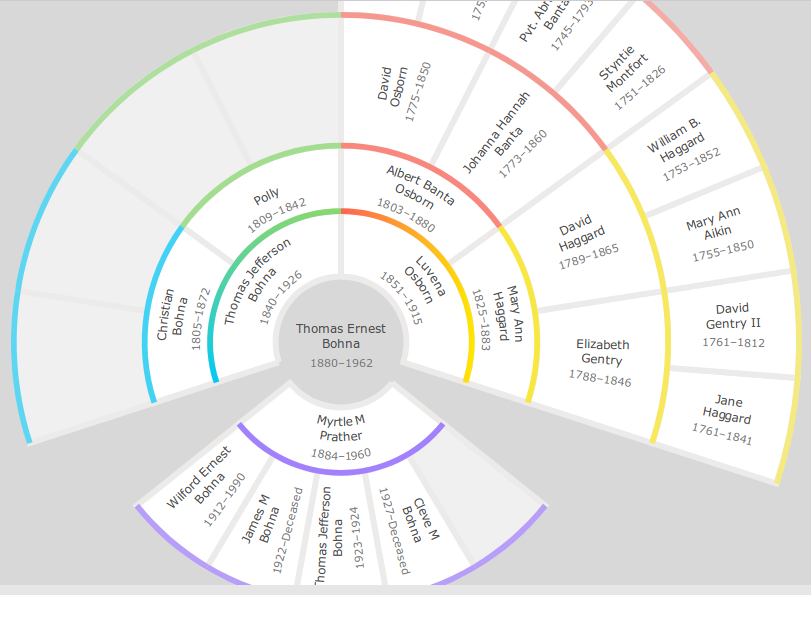
\includegraphics[width=\columnwidth]{images/familysearch/family_tree.png}
\caption{Family Tree}
\label{fig:source-linker}
\end{figure}

\section*{Security Force Monitor Implementation}
The staff of the Security Force Monitor use news articles to build an
accurate information about the security forces active within a region
of interest, their organizational structure, and the careers of
officers within that structure.

The knowledge management system that DataMade is building with
Security Force Monitor has many of the same types of elements as
FamilySearch.com. The similarities and differences demonstrate the
requirements for this type of system.

Like FamilySearch.org, current information about an entity will be
available on a profile view. However, Security Force Monitor needs to
manage information about two types of entities: officers and
organizational units. For an officer, we will track the name,
appearances at particular places and times, membership in
organizational units and the role associated with that membership, and
the directly superordinate and subordinate officers at particular
times (Figure~\ref{fig:entity-detail}).

For organizational units, we will record the name, observations of the
unit or members of the units at particular places and times, direct
superunit and subunits of the units, and the history of commanding
officers of the unit.

\begin{figure}[h]
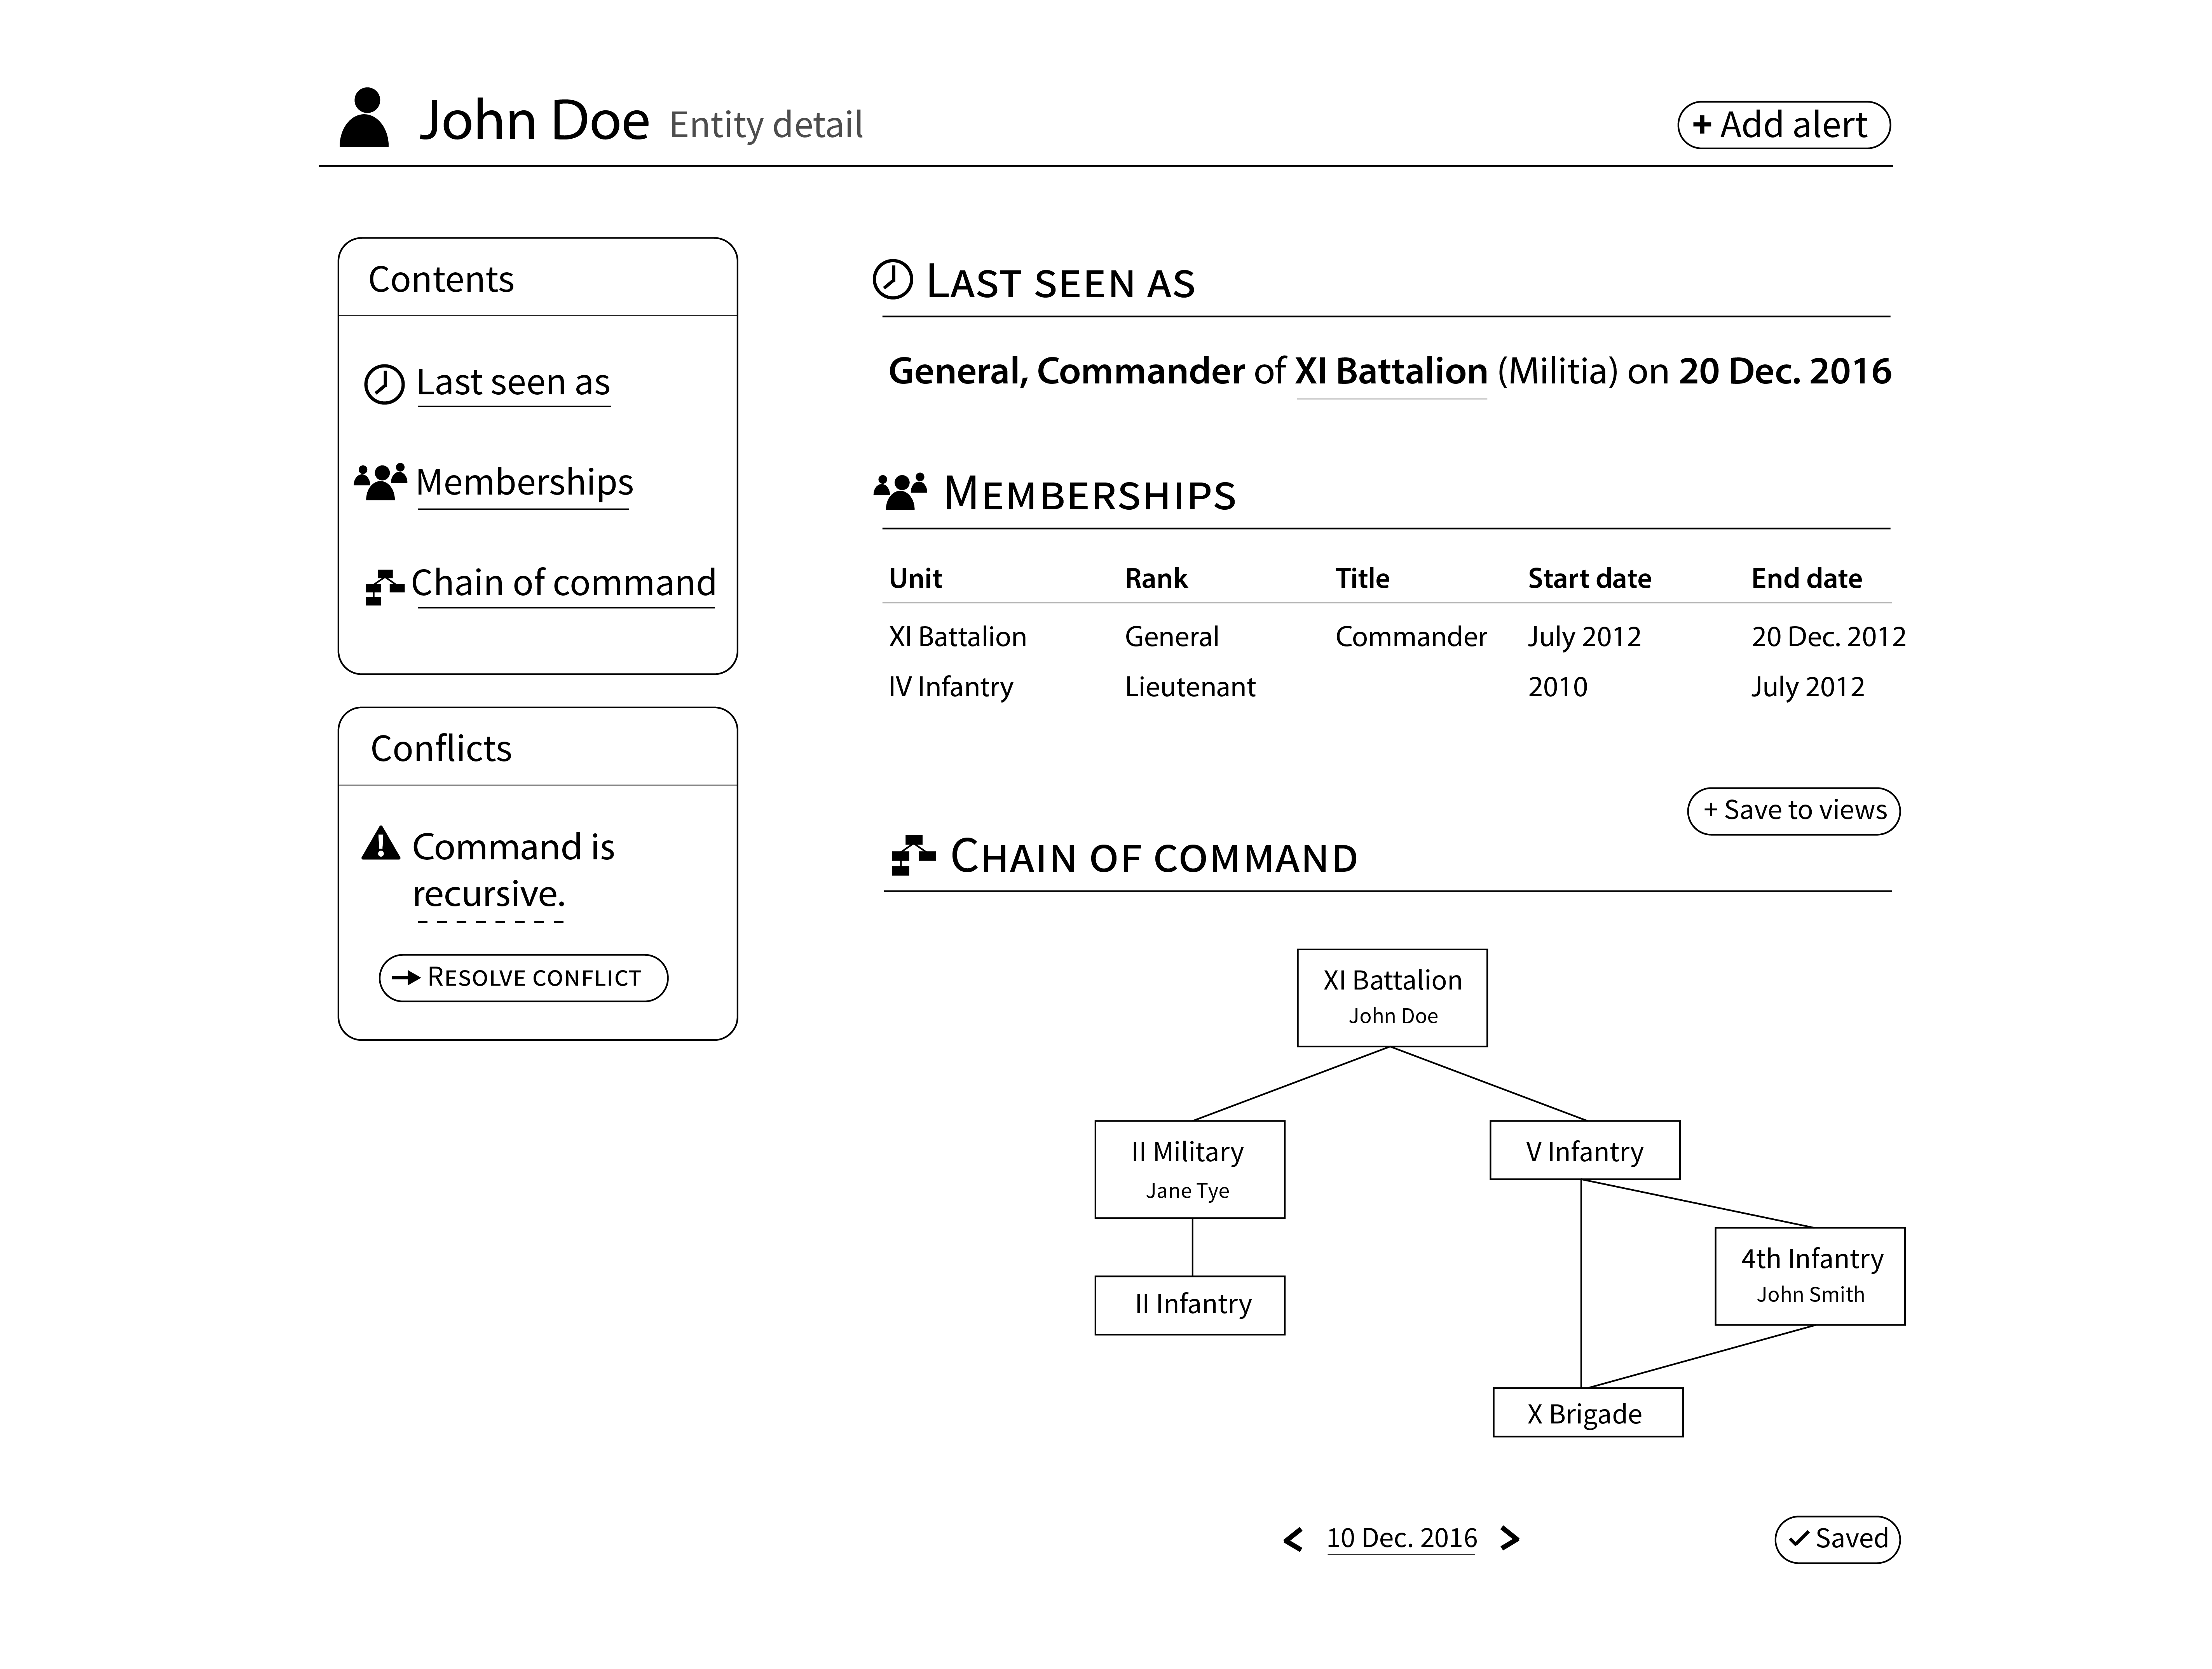
\includegraphics[width=\columnwidth]{images/sketches/entity-detail.png}
\caption{Profile View}
\label{fig:entity-detail}
\end{figure}

Unlike Family Search, the Security Force Monitor workflow is flow is
not sharply divided between source document acquisition and indexing
on one hand versus claim management on the other.

A key task for staff is to extract information about an relevant
people and organizations from a news item. From the user's
perspective, they are directly connecting the information in the news
article to an existing profile page, but the system actually records
this information as two distinct sets of claims. First, this source
document mentions an entity with this name, i.e. ``XI
Battalion''. Second, this name references the entity known to this
system as ``12135117'' Later, if we decide that this name actually
refers to some other batallion, we can re-use the first half of the
work done by the staff.

The user interface for this extraction will mainly through the
annotation of source documents (Figure~\ref{fig:new-entities}). The user
will select text from a news item that refers to an entity of
interest, which will prompt the user to record a claim. The universe
of possible types of claims is constrained by the system but can
include claims like ``A unit called `XI Batallion' operates in the
`Southern Province' as of the time of this news article'' or ``The `XI
Batallion` is commanded by `John Doe' as of the time of this news
article'. Representations of these claims will appear on profile pages
and be linked back to the source document.

\begin{figure}[h]
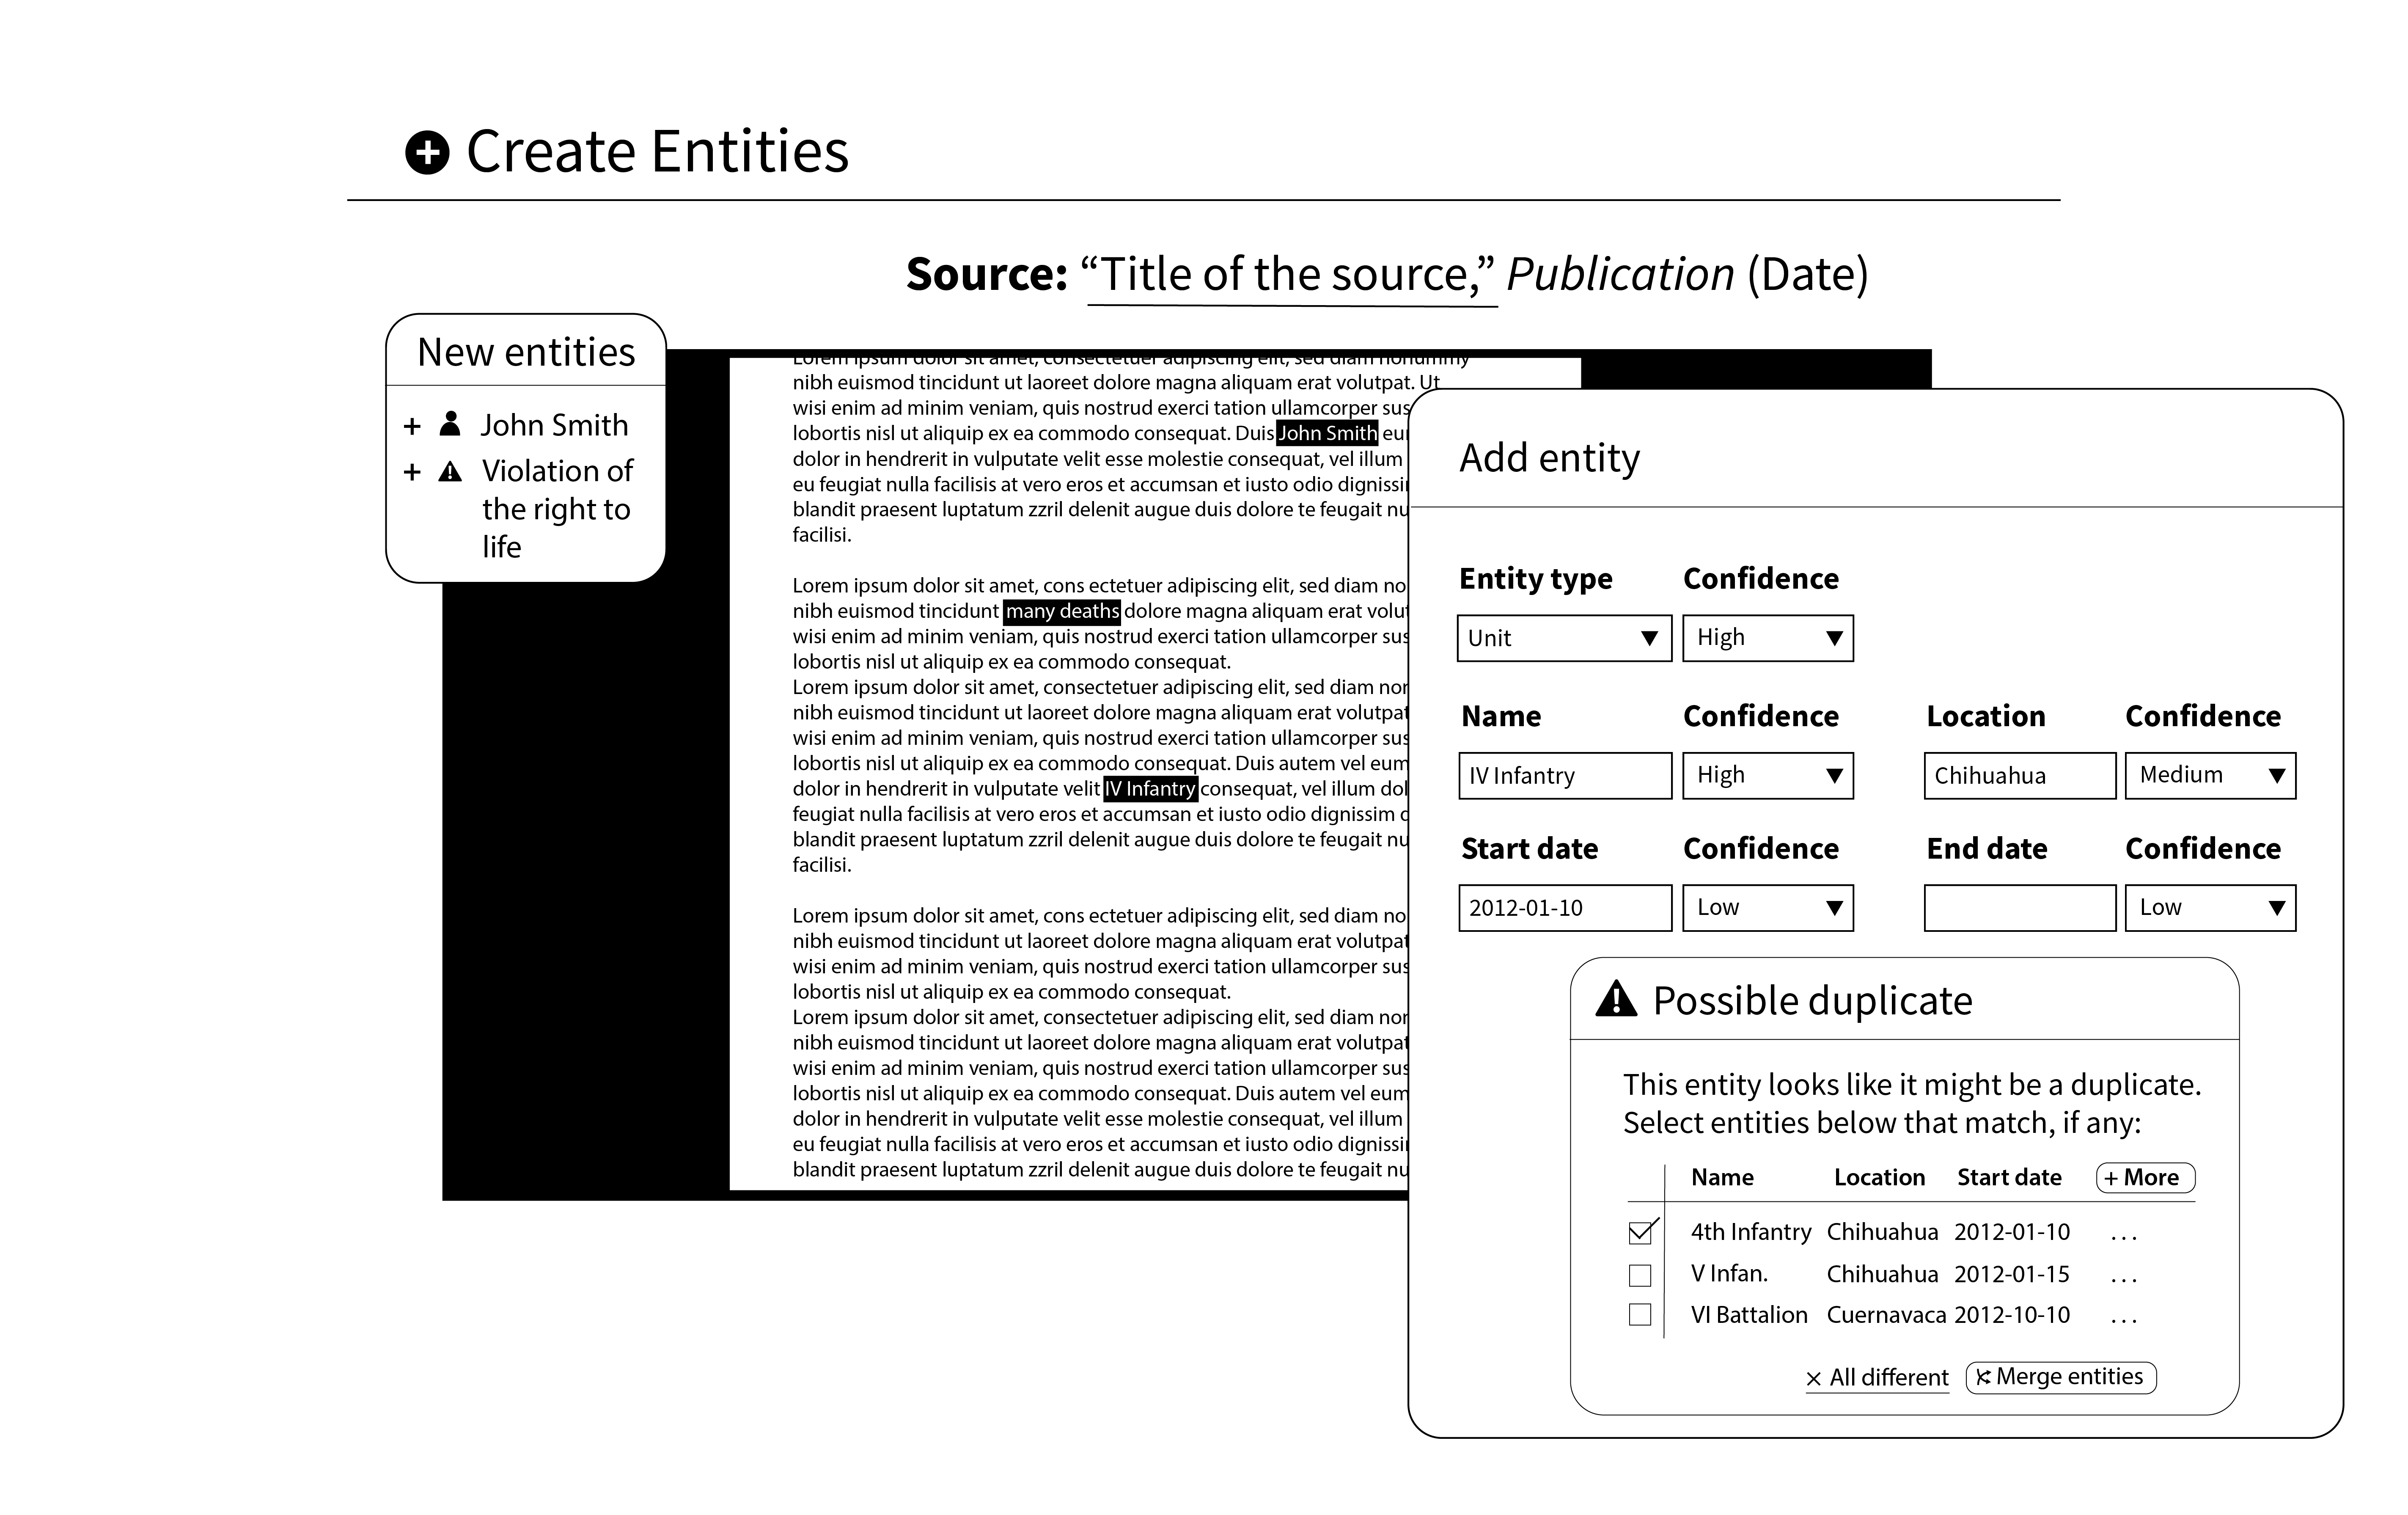
\includegraphics[width=\columnwidth]{images/sketches/new-entities.png}
\caption{Source Extraction}
\label{fig:new-entities}
\end{figure}

The Security Force Monitor staff will often be focused on the same
area and security forces. Indivividual users need means to track how
the changes other users are making directly or indirectly effect the
entities they are responsible for. Users will be able to ``watch''
entities and be notified about changes that impinge on those entities
as well as their own recent actions (Figure~\ref{fig:dashboard}).

\begin{figure}[h]
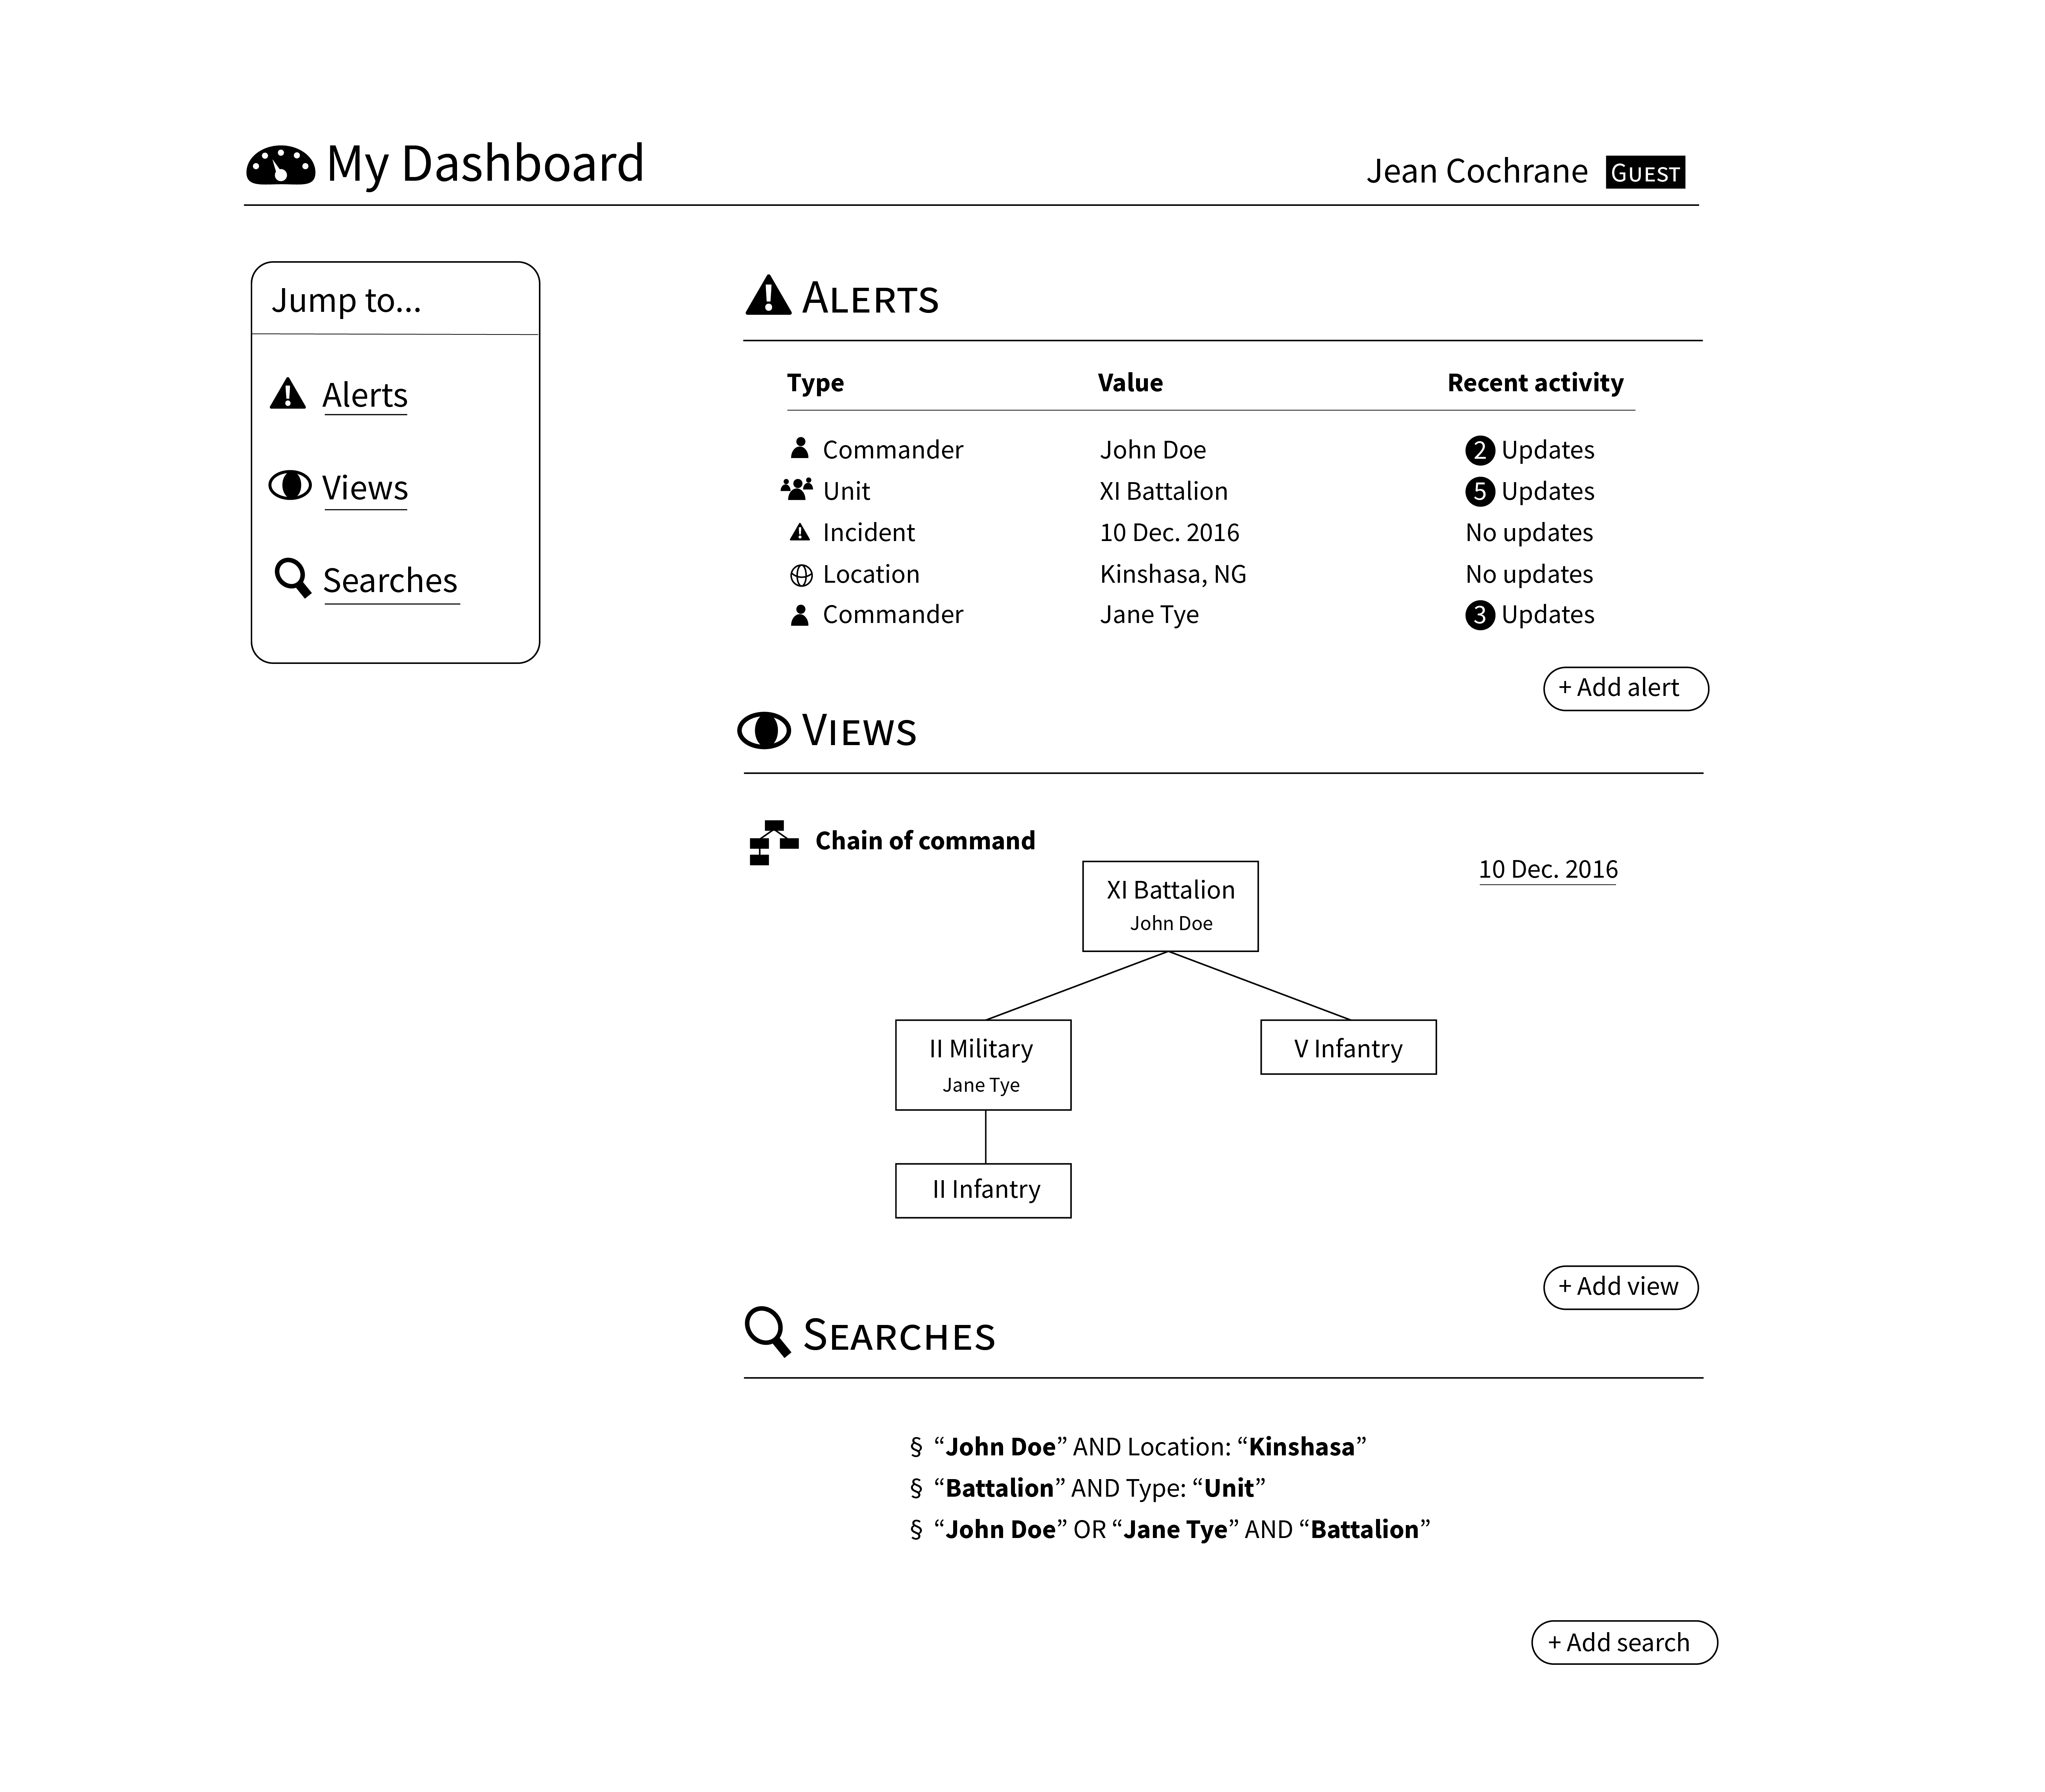
\includegraphics[width=\columnwidth]{images/sketches/dashboard.png}
\caption{Source Extraction}
\label{fig:dashboard}
\end{figure}



\subsection{Uncertainty in Claims}
Since the work of Lotfi Zadeh [TODO: Citation!], the worlds of logic
and computer science have reckoned with uncertainty and partial truth
using computation-friendly tools. Incorporating some measure of
uncertainty into any claims (and enabling the adjustment of this level
of uncertainty as new information is added) is an important part of
claims management as well as detecting and reconciling conflicting
claims.


Recording (and modifying) the reporter's uncertainty about a claim
only records half of the uncertainty that is possible in the
reportage/world-being-reported-on system. In addition to the
uncertainty in knowledge, which can be modeled, there is uncertainty
in the world.

As a few examples, the officer who has formal authority over a
security force unit may not be the person who has effective
leadership. Between units, formally subordinate units may act with
autonomy than officially granted. The scope of authority between
political commisars and commanding officers often overlap and are
contested. Between security units, particularly those in forces that
are blend of separate chains of commands, as in multinational
commands, the formal chain of command can change rapidly and sometimes
not unitary.

These occasions, where authority, leadership, and command are
ambiguous or contested make certain types of abuses more likely, and
indeed ambiguity is often created by leadership to protect themselves
from a policy of violence and oppression. This type of uncertainty
also needs to modeled.

\section{Differences in Implementation}

Different knowledge domains have different research needs. When
implementing a machine-assisted dossier, trade-offs will have to be made
between the flexibility afforded to individual researchers and the
usability of the system for a wider collective. Specific implementations
of the system we propose will vary in the degree to which they permit
the following features:

\begin{description}
  \item [Conflict resolution] It may be beneficial to some systems to
    allow conflicting claims about entities or attributes to coexist,
    and to expose these conflicts to users. Other systems will want
    to enforce a unitary vision of the world.

  \item [Custom attachments] Researchers may wish to collect unstructured
    data in the system, in order to keep track of information they might
    need at a later date, or to pursue promising lines of inquiry that
    have not yet proven to be valuable to the collective.

  \item [Interface between document collection and claim management] When
    conflicting claims get resolved, it is likely that logic will
    want to propagate down toward decisions made in the lower levels
    of document collection. Some systems will want to adjust these lower
    levels automatically; others will want to expose inconsistencies to
    researchers through the system interface, to allow them to adjudicate
    the claims. Still others may wish to permit logical inconsistencies.
\end{description}

\section{Conclusion}
We have discussed what we see as necessary for a knowledge system that
helps journalists and other types of researchers do their research
and, as a byproduct, produce reusable knowledge for themselves and
their colleagues. In particular, we have discussed the requirements
for managing claims about the world and discussed possible
implementations to satisfy those requirements.

While it is useful to describe clearly what those requirements are,
there is still significant opportunity left to make it easier to build
these types of systems in the future. As we mentioned, the document
management and indexing systems are fairly mature and modular. We
believe that it will be possible to see similar development in the
work of claim management. 














\end{document}

